% See exam.cls and examdoc.tex for the license information
\documentclass[12pt, answers]{exam}

\usepackage{amssymb}
\usepackage{makeidx}
\usepackage{amsmath}
\usepackage{graphicx}
\usepackage{caption}
\usepackage{tabulary}
\usepackage{color}
\usepackage{multicol}
\usepackage{float}
%\usepackage{multirow}
%\usepackage{enumerate}

\usepackage{array}
\newcolumntype{C}[1]{>{\centering\let\newline\\\arraybackslash\hspace{0pt}}m{#1}}

\addpoints

% In case we're not using hyperref.sty:
\providecommand{\texorpdfstring}[2]{#1}
% The following can be used in \section commands
% without generating pdf warnings:
\newcommand{\bs}{\texorpdfstring{\char`\\}{}}

\makeindex

\newcommand{\indc}[1]{\index{#1@\texttt{\char`\\#1}}}
\newcommand{\indcsub}[2]{\index{#1@\texttt{\char`\\#1}!#2}}
\newcommand{\indcstart}[1]{\index{#1@\texttt{\char`\\#1}|(}}
\newcommand{\indcstop}[1]{\index{#1@\texttt{\char`\\#1}|)}}

\newcommand{\indt}[1]{\index{#1@\texttt{#1}}}
\newcommand{\indtsub}[2]{\index{#1@\texttt{#1}!#2}}
\newcommand{\indtstart}[1]{\index{#1@\texttt{#1}|(}}
\newcommand{\indtstop}[1]{\index{#1@\texttt{#1}|)}}

\extraheadheight{-.4in}

\pagestyle{headandfoot}
%\extraheadheight{.2 in}
\firstpageheader{}{}{}
\runningheader{}{}{}
\firstpagefooter{}{Local alignment}{Page \thepage\ of \numpages}
\firstpagefootrule
\runningfooter{}{Local alignment}{Page \thepage\ of \numpages}
\runningfootrule

%---------------------------------------------------------------------

\shadedsolutions
%\noprintanswers
\definecolor{SolutionColor}{rgb}{0.8,0.9,1}

\setcounter{section}{3}

\begin{document}

\section{Exercise solutions -- Local alignment}

%---------------------------------------------------------------------
\begin{questions}

%%% Question 1
\question \textbf{Local alignment with DP}
  
The DP algorithm can be used to identify optimal local alignments. Assume the scoring scheme as match: 1, mismatch: -1, and gap penalty: 1.

\vspace{0.1 in}

\begin{parts}

%% (a)
  \part Complete the DP table to find the optimal local alignment.

\begin{figure}[h]
      \centering
      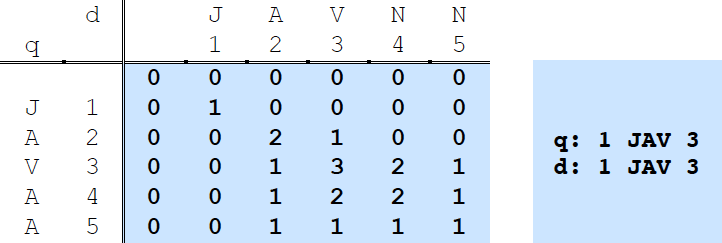
\includegraphics[width=0.7 \textwidth]{fig04/local_dp_solution.png}
\end{figure}

%% (b)
\part Backtrack from $H_{9,6}$ and write down the local alignment.  

\begin{figure}[h]
      \centering
      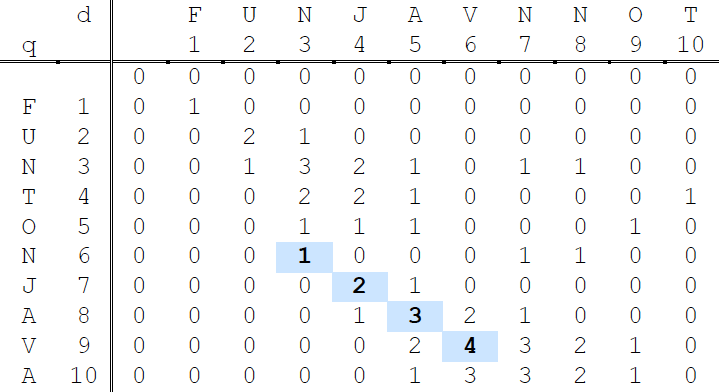
\includegraphics[width=0.75 \textwidth]{fig04/local_dp_backtrack_solution.png}
\end{figure}

\begin{solution}[0.75 in]
\begin{verbatim}
  q: 6 NJAV 9
  d: 3 NJAV 6
\end{verbatim}
\end{solution}

\end{parts}


\newpage

%%% Question 2
\question \textbf{Dot matrix}
  
A dot matrix is one of the simplest methods to identify local alignments. 

\vspace{0.1 in}

\begin{parts}

%% (a)
  \part Fill the table with dots.

\begin{figure}[h]
      \centering
      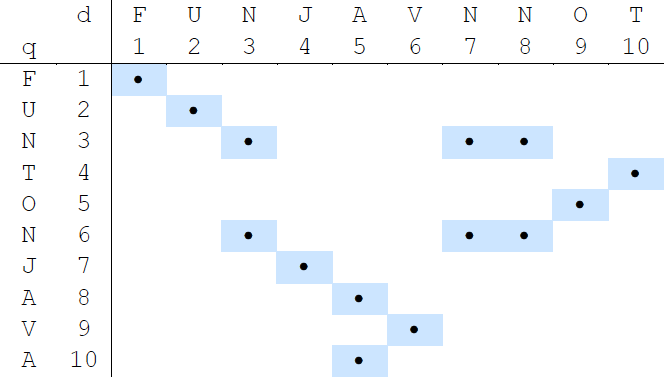
\includegraphics[width=0.7 \textwidth]{fig04/dot_matrix_solution.png}
\end{figure}

%% (b)
\part Identify all segment pairs with at least 3 contiguous dots along diagonals.

\begin{solution}[0.75 in]
\begin{verbatim}
  q: 1 FUN 3        q: 6 NJAV 9
  d: 1 FUN 3        d: 3 NJAV 6
\end{verbatim}
\end{solution}

%% (c)
\part Identify all segment pairs with at least 3 contiguous dots along aniti-diagonals.

\begin{solution}[0.75 in]
\begin{verbatim}
  q: 4 TON 6
  d: 8 NOT 10
\end{verbatim}
\end{solution}

\end{parts}



\end{questions}
%---------------------------------------------------------------------
       
\end{document}

